%\documentclass[first,firstsupp,handout,compress,notes,navigation]{ETHclass} 
%\documentclass[first,firstsupp,handout,lastsupp]{ETHclass} 
\documentclass[first,firstsupp,lastsupp,handout,last,hyperref,table]{ETHclass} 
%\documentclass[first,firstsupp]{ETHclass}
\usepackage{etex}

\usepackage{adjustbox}
\usepackage{amsmath}
\usepackage{amssymb}
\usepackage{animate}
\usepackage{booktabs}
\usepackage{charter}
\usepackage{etoolbox}
\usepackage{ifthen}
\usepackage{longtable}
\usepackage{mathrsfs}
\usepackage{multicol}
\usepackage{pgf}
\usepackage{ragged2e}
\usepackage{standalone}
\usepackage[caption=false]{subfig}
\usepackage{tabularx}
\usepackage{tikz}
\usepackage{verbatim}
\usepackage{xcolor}
\usepackage{hyperref}




\setbeamertemplate{navigation symbols}{}
\usetikzlibrary{arrows,decorations.pathreplacing,positioning,shapes,shadows}

%\usepackage[style=numeric-comp]{biblatex}

%\usepackage{lipsum}

%\usetikzlibrary{fit}
\usetikzlibrary{arrows}
\usetikzlibrary{trees}

% Options for beamer:
%
% 9,10,11,12,13,14,17pt  Fontsizes
% 
% compress: navigation bar becomes smaller
% t       : place contents of frames on top (alternative: b,c)
% handout : handoutversion
% notes   : show notes
% notes=onlyslideswithnotes
%
%hyperref={bookmarksopen,bookmarksnumbered} : Needed for menues in
%                                             acrobat. Also need
%                                             pdftex as option or 
%                                             compile with
% pdflatex '\PassOptionsToPackage{pdftex,bookmarksopen,bookmarksnumbered}{hyperref} \input{file}'

%\usepackage{beamerseminar}
%\usepackage[accumulated]{beamerseminar}
                                % remove ``accumulated'' option
                                % for original behaviour
%\usepackage{beamerbasenotes}
%\setbeamertemplate{note page}[plain] 
%\setbeameroption{notes on second screen}

%\setbeamertemplate{note page}[plain] 
\setbeamertemplate{note page}{\ \\[.3cm]
\textbf{\color{blue}Notes:}\\%[0.1cm]
{\footnotesize %\tiny
\insertnote}}
%\setbeameroption{notes on second screen}


%\setbeamertemplate{navigation symbols}{} % suppresses all navigation symbols:
 \setbeamertemplate{navigation symbols}[horizontal] % Organizes the navigation symbols horizontally.
% \setbeamertemplate{navigation symbols}[vertical] % Organizes the navigation symbols vertically.
% \setbeamertemplate{navigation symbols}[only frame symbol] % Shows only the navigational symbol for navigating frames.

\setlayoutscale{0.5}
\setparametertextfont{\scriptsize}
\setlabelfont{\scriptsize}

% \useoutertheme[subsection=false]{miniframes}
% \usepackage{etoolbox}
% \makeatletter
% \patchcmd{\slideentry}{\advance\beamer@xpos by1\relax}{}{}{}
% \def\beamer@subsectionentry#1#2#3#4#5{\advance\beamer@xpos by1\relax}%
% \makeatother

% \makeatletter
%     \newenvironment{withoutheadline}{
%        \setbeamertemplate{headline}{%
% \vspace{15pt}
% }
%     }{}
% \makeatother

\makeatletter
    \newenvironment{withoutheadline}{
         \setbeamertemplate{headline}{%
\vspace{35pt}
}
        %\def\beamer@entrycode{\vspace*{-1.5\headheight}}
    }{}
\makeatother

\newcommand{\Cross}{$\mathbin{\tikz [x=1.4ex,y=1.4ex,line width=.2ex, red] \draw (0,0) -- (1,1) (0,1) -- (1,0);}$}%

\newcommand{\Checkmark}{$\color{green}\checkmark$}

\setbeamerfont{subsection in toc}{size=\tiny}

\makeatletter
\patchcmd{\beamer@sectionintoc}
  {\vfill}
  {\vskip1.5\itemsep}
  {}
  {}
\makeatother  

\setbeamertemplate{frametitle continuation}{}

\setbeamertemplate{bibliography entry title}{}
\setbeamertemplate{bibliography entry author}{}
\setbeamertemplate{bibliography entry location}{}
\setbeamertemplate{bibliography entry note}{}

\setbeamercolor*{bibliography entry title}{fg=black}
\setbeamercolor*{bibliography entry author}{fg=black}
\setbeamercolor*{bibliography entry location}{fg=black}
\setbeamercolor*{bibliography entry note}{fg=black}
% and kill the abominable icon
%\setbeamertemplate{bibliography item}{\color{forestgreen}$\blacktriangleright$}
\setbeamertemplate{bibliography item}{\insertbiblabel}
%\setbeamertemplate{bibliography item}{\theenumiv}

\newcommand{\highlightred}[1]{%
  \colorbox{red!50}{$\displaystyle#1$}}
  
\newcommand{\highlightyellow}[1]{%
  \colorbox{yellow!50}{$\displaystyle#1$}}
  
\newcommand{\highlightgreen}[1]{%
  \colorbox{green!50}{$\displaystyle#1$}}

\AtBeginSection[]{
  \begin{frame}
  \vfill
  \centering
  \begin{beamercolorbox}[sep=8pt,center,shadow=true,rounded=true]{title}
    \usebeamerfont{frametitle}
\includegraphics[width=2ex]{freccia_trasparente_verde_foresta.png}\hspace{.5ex}~{\LARGE \textsc{\bfseries \insertsectionhead}}\par%
  \end{beamercolorbox}
  \vfill
  \end{frame}
}

\hyphenpenalty=5000
\tolerance=1000

\graphicspath{{figures/}}

\newenvironment{system}%
{\left\lbrace\begin{array}{@{}l@{}}}%
{\end{array}\right.}

\newenvironment{subsystem}%
{\left\lgroup\begin{array}{@{}l@{}}}%
{\end{array}\right.}

\defbeamertemplate*{title page}{customized}[1][]
{
\usebeamerfont{subtitle}
\usebeamercolor[fg]{subtitle}

\vspace{-1.25cm}

{\flushleft
 \usebeamerfont{title}{\inserttitle}\par
}
\vspace{-.25cm}
{\flushleft
 \usebeamerfont{subtitle}{\small \insertsubtitle} \par
}

\vspace{-.5cm}

{\flushright
\setbeamercolor{author}{bg=white,fg=Red}
\usebeamerfont{author}{\footnotesize \insertauthor} \par}

\vspace{-.2cm}

{\flushright
\usebeamerfont{institute}{\tiny \insertinstitute}\par }

\vspace{.2cm}

{\centering
\usebeamerfont{date}{\scriptsize \insertdate} \par }

\vspace{0.2in}

%%----------------------------------------------------------------------------------------------%
%%                                          INPUT PARAMETERS
%%----------------------------------------------------------------------------------------------%
%
%\def\Rf{1}
%\def\Vff{0.5}
%\def\tratio{0.75}
%\def\meshfacone{0.2}
%\def\meshfactwo{0.75}
%\def\meshfacthree{0.5}
%\def\thetavalue{45}
%\def\deltatheta{15}
%
%%----------------------------------------------------------------------------------------------%
%%                               Definition of dependent parameters
%%----------------------------------------------------------------------------------------------%
%
%\def\pivalue{3.141592653589793238462643383279502884197169399375105820974944592307816406286}
%\pgfmathsetmacro\sqrttwo{sqrt(2)}
%
%\newcommand{\half}[1]{
%       0.5*#1
%       }
%
%\pgfmathsetmacro\l{0.5*\Rf*sqrt(\pivalue/\Vff)}
%
%\def\domlim{1.28*\l}
%\def\loadlim{1.197*\l}
%\def\loadlabel{0.2*\Rf}
%\def\cornerlabel{1.077*\l}
%
%\def\thetabot{\thetavalue-\deltatheta}
%\def\thetaup{\thetavalue+\deltatheta}
%
%\def\thetahalfbot{\thetavalue-0.5*\deltatheta}
%\def\thetahalfup{\thetavalue+0.5*\deltatheta}
%
%\def\thetaround{360+\thetavalue-\deltatheta}
%\def\thetadraw{0.25*\thetavalue}
%
%\def\xM{0.9*\costheta*\Rf}
%\def\yM{0.9*\sintheta*\Rf}
%
%\pgfmathsetmacro\cosfourtyfive{cos(45)}
%\pgfmathsetmacro\sinfourtyfive{sin(45)}
%
%\pgfmathsetmacro\costheta{cos(\thetavalue)}
%\pgfmathsetmacro\sintheta{sin(\thetavalue)}
%
%\pgfmathsetmacro\costhetabot{cos(\thetabot)}
%\pgfmathsetmacro\sinthetabot{sin(\thetabot)}
%
%\pgfmathsetmacro\costhetaup{cos(\thetaup)}
%\pgfmathsetmacro\sinthetaup{sin(\thetaup)}
%
%\pgfmathsetmacro\costhetahalfbot{cos(\thetahalfbot)}
%\pgfmathsetmacro\sinthetahalfbot{sin(\thetahalfbot)}
%
%\pgfmathsetmacro\costhetahalfup{cos(\thetahalfup)}
%\pgfmathsetmacro\sinthetahalfup{sin(\thetahalfup)}
%  
%\pgfmathsetmacro\yloadarrowone{\l+(\loadlim-\l)*0.2}
%\pgfmathsetmacro\yloadarrowtwo{\l+2*(\loadlim-\l)*0.2}
%\pgfmathsetmacro\yloadarrowthree{\l+3*(\loadlim-\l)*0.2}
%\pgfmathsetmacro\yloadarrowfour{\l+4*(\loadlim-\l)*0.2}
%
%\pgfmathsetmacro\ILsquared{(\costhetabot-\costhetaup)*(\costhetabot-\costhetaup)+(\sinthetabot-\sinthetaup)*(\sinthetabot-\sinthetaup))}
%\pgfmathsetmacro\IMsquared{(\costhetabot-0.9*\costheta)*(\costhetabot-0.9*\costheta)+(\sinthetabot-0.9*\sintheta)*(\sinthetabot-0.9*\sintheta)}
%\pgfmathsetmacro\IL{sqrt(\ILsquared)}
%\pgfmathsetmacro\IM{sqrt(\IMsquared)}
%\pgfmathsetmacro\angleM{asin(0.5*\IL/\IM)}
%
%\def\crackstartangle{\thetavalue-\angleM}
%\def\crackstopangle{\thetavalue+\angleM}
%
%\pgfmathsetmacro\meshradiusone{\meshfactwo*\Rf}
%\pgfmathsetmacro\meshradiustwo{\Rf+\meshfacthree*(\l-\Rf)}

%\begin{beamercolorbox}[sep=1em,wd=1.1\textwidth,ht=3cm,dp=3cm,right]{white}
%\usebeamerfont{title} {\huge \inserttitle}\par
%\usebeamerfont{subtitle} {\insertsubtitle}
%\end{beamercolorbox}
}


\begin{document}
\setbeamertemplate{caption}{\raggedright\insertcaption\par}

\title{\textsc{RVE-based Micromechanical Analysis of Fiber-Matrix Debonding in Thin Ply FRPC Laminates}}
\author{ L. Di Stasio$^{1,2}$, Z. Ayadi$^{1}$, J. Varna$^{2}$}
%\institute{ Science et Ing\'enierie des Mat\'eriaux et M\'etallurgie (SI2M), Institut Jean Lamour, Nancy, France\\Department of Engineering Sciences and Mathematics, Division of Materials Science, Lule\aa\ University of Technology, Lule\aa, Sweden}
\institute{$^{1}$EEIGM, Universit\'e de Lorraine, Nancy, France\\$^{2}$Division of Materials Science, Lule\aa\ University of Technology, Lule\aa, Sweden}
\date{DocMASE Summer School, Lule\aa , 2016}

\begin{frame}[plain]
    \titlepage
\end{frame}

\begin{withoutheadline}
\begin{frame}
\frametitle{Outline}
\justifying
\vspace*{-0.5cm}
% \tableofcontents[hidesubsections]
% \begin{multicols}{2}
% \tableofcontents[hidesubsections]
% \end{multicols}
% \begin{columns}[t]
%         \begin{column}{.5\textwidth}
%             \tableofcontents[sections={1-2}]
%         \end{column}
%         \begin{column}{.5\textwidth}
%             \tableofcontents[sections={3-6}]
%         \end{column}
%     \end{columns}
% \end{frame}
\tableofcontents[hidesubsections]
\end{frame}
\end{withoutheadline}

%\note{}

%\begin{frame}
%\pagediagram
%\end{frame}
%% \note{}

\section{Introduction to Thin Ply FRP Laminates}

\subsection{What are composite materials?}

\begin{frame}
\frametitle{What are composite materials?}
%\vspace{1cm}
\centering
\begin{figure}[!h]
\centering
\subfloat[\scriptsize Egyptian mud bricks.\label{fig:brick}]{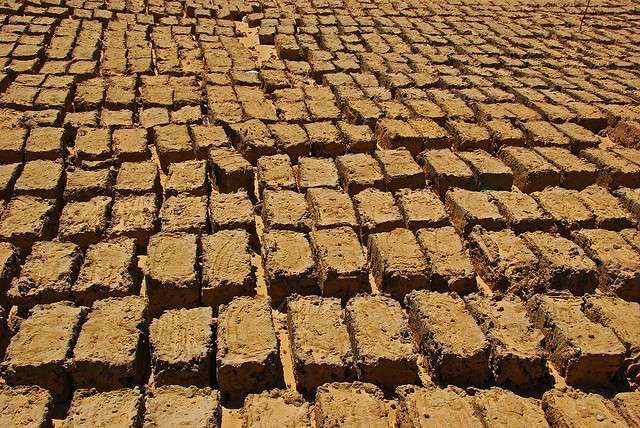
\includegraphics[height=0.45\textheight,width=0.45\textwidth]{egyptian_mud_bricks.jpg}}\quad
\subfloat[\scriptsize Fiber reinforced polymer (FRP) laminate.\label{fig:composite-lam}]{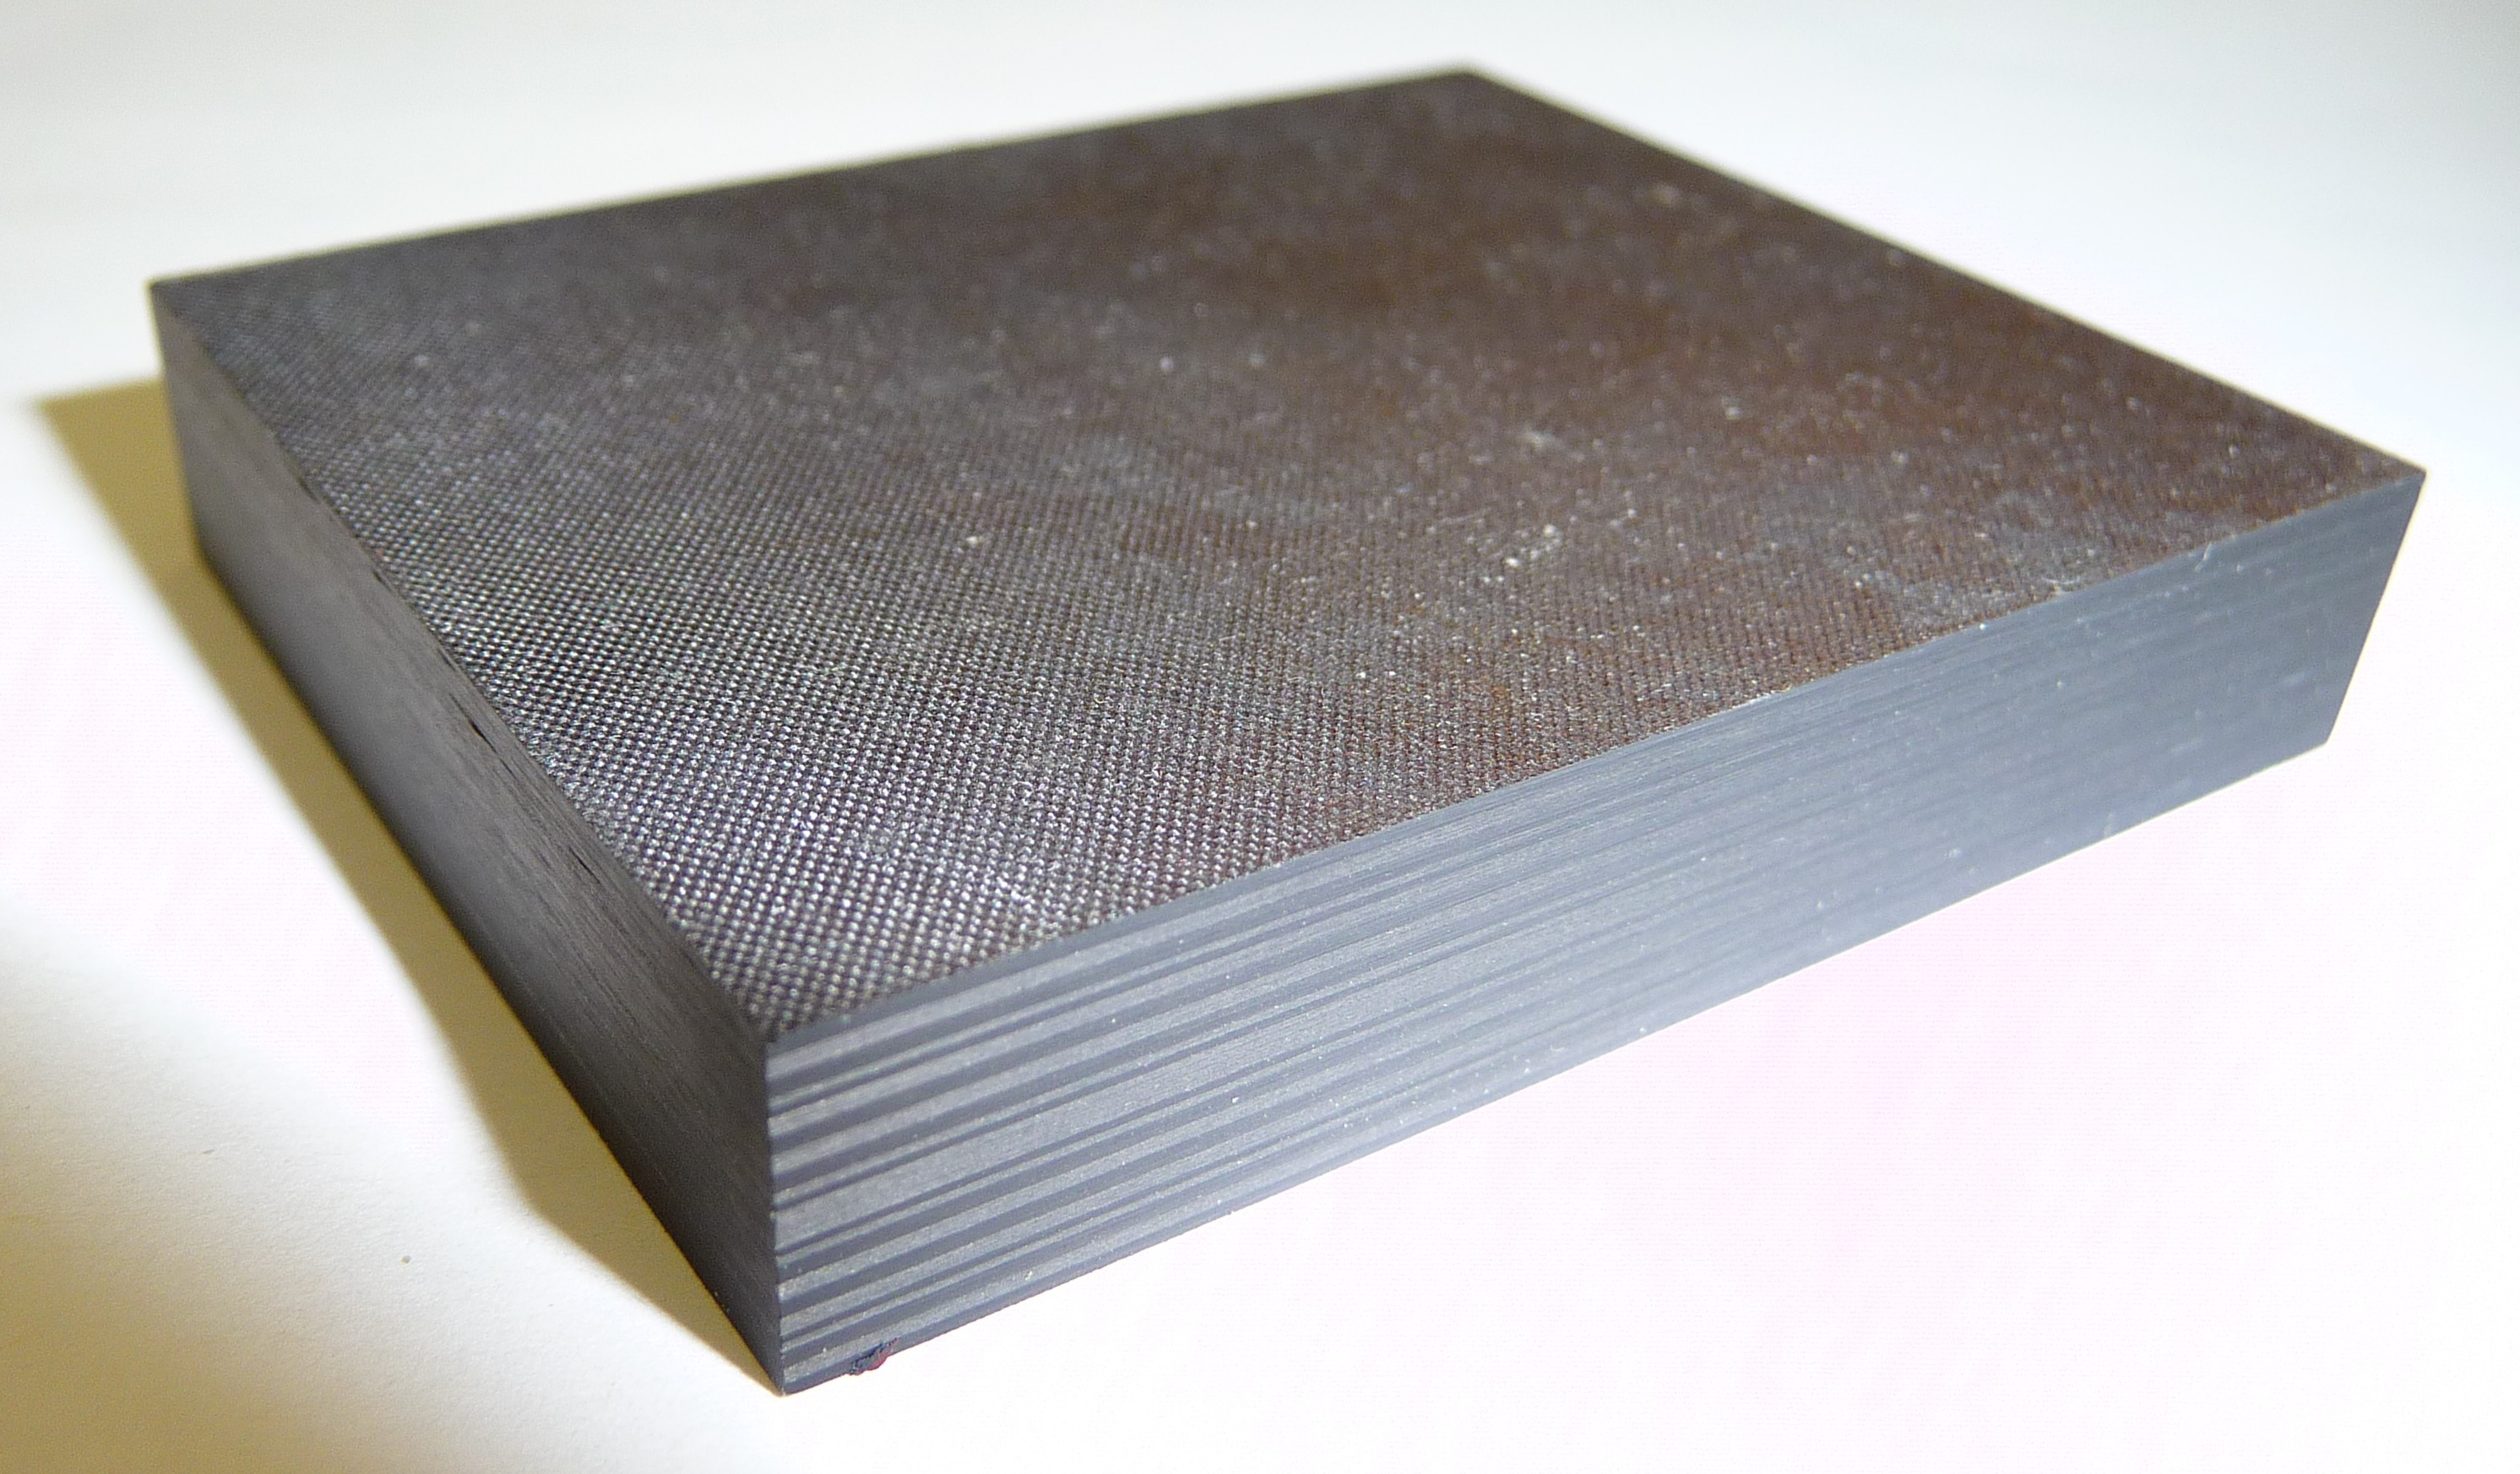
\includegraphics[height=0.45\textheight,width=0.45\textwidth]{Composite_laminate_specimen.jpg}}
  %\caption{Single RVE model.}
  \label{fig:composites}
\end{figure}
\end{frame}

\note{\begin{itemize}
    \item Composite materials represent a wide class
    \item A precise definition can be difficult
    \item Ancient example: Egyptian mud bricks. Straw and mud: randomly arranged short fibers in continuous matrix in modern terminology.
    \item Modern example: FRP laminates. Carbon fibers in polymeric matrix: regularly arranged long fibers in continuous matrix.
\end{itemize}}

\begin{frame}
\frametitle{What are composite materials?}
%\vspace{1cm}
\centering
\begin{quote}
More important than any one new application is the new 'materials' concept itself. It marks a shift from concern with substances to concern with structures, a shift from artisan to scientist as man's artificer, a shift from chemistry to physics as the basic discipline, and a shift, above all, from the concrete experience of the workshop to abstract mathematics, a shift from starting with what nature provides to what man wants to accomplish.
\end{quote}

Peter Drucker, \textit{The Age of Discontinuity}, 1969.
\end{frame}

\note{\begin{itemize}
    \item He was not a materials scientist, but management thinker
    \item However, he got some point right
    \item shift to structures
    \item shift to mathematics
    \item shift to what man wants to accomplish
\end{itemize}}

\subsection{Thin Ply FRP Laminates: a primer}

\begin{frame}
\frametitle{Fiber Tows and Prepreg}
%\vspace{1cm}
\centering
\begin{figure}[!h]
\centering
\subfloat[\scriptsize Carbon fiber tow.\label{fig:brick}]{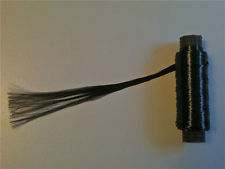
\includegraphics[height=0.45\textheight,width=0.35\textwidth]{carbon-fiber-tow.jpg}}\quad
\subfloat[\scriptsize Carbon fiber prepreg.\label{fig:composite-lam}]{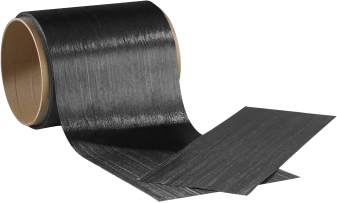
\includegraphics[height=0.45\textheight,width=0.55\textwidth]{prepreg.png}}
  %\caption{Single RVE model.}
  \label{fig:composites}
\end{figure}
\end{frame}

\note{\begin{itemize}
    \item Fibers are gathered together in tows, 6k or 12k
    \item Then used in production
    \item Commonly used intermediate stage: prepreg
    \item Prepreg: fibers laid down in a layer and pre-impregnated with resin
\end{itemize}}

\begin{frame}
\frametitle{Spread tow technology}
\vspace{-.5cm}
\centering
\begin{figure}
\centering
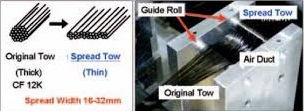
\includegraphics[width=0.8\textwidth]{spread_tow_technology_scheme}
%\caption{A schematic representation of the technology.}
\label{fig:design_workflow}
\end{figure}
\end{frame}

\note{\begin{itemize}
    \item Fibers are spread out
    \item Layers produced with this technology are very thin: a few multiples of fiber radius
\end{itemize}}

\section{The rationale of the project}

\subsection{Problem}

\begin{frame}
\frametitle{Problem}
\begin{itemize}
    \item Strength advantages due to a positive size-effect with decreasing ply thickness~\cite{RobinAmacherWayneSmithClemensDransfeldJohnBotsis2014}
    \item Good experimental knowledge
    \item Predictive capability, especially for failure, is scarce (WWFE-II and WWFE-III)~\cite{RalfCuntze}
\end{itemize}
\end{frame}

\subsection{Objective}

\begin{frame}
\vspace*{-1cm}
\frametitle{Objective \& Method}
\begin{equation}
G_{*c}=G_{*c}\left(geometry, fiber orientation, elastic\ properties\right)
\end{equation}
\begin{itemize}
    \item Micromechanical analysis
    \item Design of Reference Volume Element (RVE)
    \item Finite Element Simulation
\end{itemize}
\end{frame}

\section{The model}

\subsection{Geometries, loads and boundary conditions}

\begin{frame}
\frametitle{Single RVE model}
\vspace{-0.75cm}
\centering
\begin{figure}[!h]
\centering
    \includestandalone[height=0.7\textheight]{singleRVE_cc}%     without .tex extension
  % or use \input{mytikz}
  \caption{\scriptsize Initial state of single RVE model: crack closed in the radial direction.}
  \label{fig:singleRVE_onlycc}
\end{figure}
\end{frame}

\begin{frame}
\frametitle{Bounded RVE model}
\vspace{-0.75cm}
\centering
\begin{figure}[!h]
\centering
    \includestandalone[height=0.7\textheight]{boundedRVE_cc}%     without .tex extension
  % or use \input{mytikz}
  \caption{\scriptsize Initial state of bounded RVE model: crack closed in the radial direction.}
  \label{fig:boundedRVE_onlycc}
\end{figure}
\end{frame}

\begin{frame}
\frametitle{Periodic RVE model}
\vspace{-0.75cm}
\centering
\begin{figure}[!h]
\centering
    \includestandalone[height=0.7\textheight]{periodicRVE_cc}%     without .tex extension
  % or use \input{mytikz}
  \caption{\scriptsize Initial state of periodic RVE model: crack closed in the radial direction.}
  \label{fig:periodicRVE_onlycc}
\end{figure}
\end{frame}

%\begin{frame}
%\frametitle{Summary of designed geometries}
%\vspace*{-0.25cm}
%\centering
%\begin{table}[htbp]
\footnotesize
  \centering
  \small
  %\caption{Model geometries summary.}
    \begin{tabularx}{\textwidth}{cc}
    \toprule
        \midrule
    \textbf{Name} & \textbf{Number of phases}\\
     single-RVE&2\\
    \midrule
    \multicolumn{2}{X}{\textbf{Description}}\\
    \multicolumn{2}{X}{Circular fiber inside a square matrix domain.}\\
    \midrule
    \multicolumn{2}{X}{\textbf{Geometry of each phase}}\\
    \multicolumn{2}{X}{Fiber: circular; matrix: square with circular inclusion at its center.}\\
    \midrule
    \multicolumn{2}{X}{\textbf{Boundary conditions}}\\
    \multicolumn{2}{X}{Constant strain at $z=\pm l$; in order to have constant strain, the displacement has a linear functional form, i.e. $u_{x}|_{z=\pm l}=\bar{u}_{x}\frac{x}{l}$.}\\
    \midrule
    \multicolumn{2}{X}{\textbf{Imposed conditions}}\\
    \multicolumn{2}{X}{Constant displacement $u_{x}|_{z=\pm l}=\bar{u}_{x}=\bar{\varepsilon}_{x}\cdot l$ at $x=\pm l$.}\\
    \midrule
    \bottomrule
    \end{tabularx}%
  \label{tab:geom_tab1}%
\end{table}%


%\end{frame}

%\begin{frame}
%\frametitle{Summary of designed geometries}
%\vspace*{-0.25cm}
%\centering
%\begin{table}[htbp]
\footnotesize
  \centering
  \small
  %\caption{Model geometries summary.}
    \begin{tabularx}{\textwidth}{cc}
    \toprule
   \midrule
    \textbf{Name} & \textbf{Number of phases}\\
     bounded-RVE&3\\
    \midrule
    \multicolumn{2}{X}{\textbf{Description}}\\
    \multicolumn{2}{X}{Circular fiber inside a square matrix domain, bounded by two UD rectangular domains on the upper and lower side.}\\
    \midrule
    \multicolumn{2}{X}{\textbf{Geometry of each phase}}\\
    \multicolumn{2}{X}{Fiber: circular; matrix: square with circular inclusion at its center; UD: rectangular.}\\
    \midrule
    \multicolumn{2}{X}{\textbf{Boundary conditions}}\\
    \multicolumn{2}{X}{Free surface at $z=\pm l$.}\\
    \midrule
    \multicolumn{2}{X}{\textbf{Imposed conditions}}\\
    \multicolumn{2}{X}{Constant displacement $u_{x}|_{z=\pm l}=\bar{u}_{x}=\bar{\varepsilon}_{x}\cdot l$ at $x=\pm l$.}\\
    \midrule
    \bottomrule
    \end{tabularx}%
  \label{tab:geom_tab2}%
\end{table}%
%\end{frame}

%\begin{frame}
%\frametitle{Summary of designed geometries}
%\vspace*{-0.25cm}
%\centering
%\begin{table}[htbp]
\footnotesize
  \centering
  \small
  %\caption{Model geometries summary.}
    \begin{tabularx}{\textwidth}{cc}
    \toprule
    \midrule
    \textbf{Name} & \textbf{Number of phases}\\
     periodic-RVE&2\\
    \midrule
    \multicolumn{2}{X}{\textbf{Description}}\\
    \multicolumn{2}{X}{Periodically repeated unit cell, constituted by a circular fiber inside a square matrix domain.}\\
    \midrule
    \multicolumn{2}{X}{\textbf{Geometry of each phase}}\\
    \multicolumn{2}{X}{Fiber: circular; matrix: square with circular inclusion at its center.}\\
    \midrule
    \multicolumn{2}{X}{\textbf{Boundary conditions}}\\
    \multicolumn{2}{X}{Periodic boundary conditions on all sides.}\\
    \midrule
    \multicolumn{2}{X}{\textbf{Imposed conditions}}\\
    \multicolumn{2}{X}{Constant displacement $u_{x}|_{z=\pm l}=\bar{u}_{x}=\bar{\varepsilon}_{x}\cdot l$ at $x=\pm l$.}\\
    \midrule
    \bottomrule
    \end{tabularx}%
  \label{tab:geom_tab3}%
\end{table}%
%\end{frame}


\subsection{Mesh characteristics}


\begin{frame}
\frametitle{Mesh regions}
\vspace{-0.75cm}
\centering
\begin{figure}[!h]
\centering
    \includestandalone[height=0.8\textheight]{mesh_regions}%     without .tex extension
  % or use \input{mytikz}
  %\caption{Block regions of the \acrshort{rve} geometry.}
  \label{fig:mesh_regions}
\end{figure}
\end{frame}


\begin{frame}
\frametitle{Mesh parameters}
\vspace{-0.75cm}
\centering
\begin{figure}[!h]
\centering
    \includestandalone[height=\textheight]{mesh_parameters_single}%     without .tex extension
  % or use \input{mytikz}
  %\caption{Parameters for mesh generation for the single and periodic \acrshort{rve}.}
  \label{fig:mesh_param_single}
\end{figure}
\end{frame}

\begin{frame}
\frametitle{Mesh parameters}
\vspace{-0.75cm}
\centering
\begin{figure}[!h]
\centering
    \includestandalone[height=\textheight]{mesh_parameters_bounded}%     without .tex extension
  % or use \input{mytikz}
  %\caption{Parameters for mesh generation for the bounded \acrshort{rve}.}
  \label{fig:mesh_param_bounded}
\end{figure}
\end{frame}

%\begin{frame}
%\frametitle{Helical numbering}
%\vspace{-0.75cm}
%\centering
%\begin{figure}[!h]
%\centering
%    \includestandalone[height=0.7\textheight]{scheme_model3}%     without .tex extension
%  % or use \input{mytikz}
%  %\caption{\scriptsize CPE4.}
%  \label{fig:helix}
%\end{figure}
%\end{frame}

%\begin{frame}
%\frametitle{Topological transformation}
%\vspace{-0.75cm}
%\centering
%\begin{figure}[!h]
%\centering
%    \includestandalone[height=0.7\textheight]{scheme_model2}%     without .tex extension
%  % or use \input{mytikz}
%  %\caption{\scriptsize CPE4.}
%  \label{fig:topo_transf}
%\end{figure}
%\end{frame}

%\begin{frame}
%\frametitle{Elements}
%\vspace{-0.75cm}
%\centering
%\begin{figure}[!h]
%\centering
%    \includestandalone[height=0.7\textheight]{abaqus_cpe4}%     without .tex extension
%  % or use \input{mytikz}
%  \caption{\scriptsize CPE4.}
%  \label{fig:cpe4}
%\end{figure}
%\end{frame}

%\begin{frame}
%\frametitle{Elements}
%\vspace{-0.75cm}
%\centering
%\begin{figure}[!h]
%\centering
%    \includestandalone[height=0.7\textheight]{abaqus_cpe8}%     without .tex extension
%  % or use \input{mytikz}
%  \caption{\scriptsize CPE8.}
%  \label{fig:cpe8}
%\end{figure}
%\end{frame}

\subsection{Types of analysis}

\begin{frame}
\frametitle{Features}
\vspace*{-0.25cm}
\centering
\begin{sidewaystable}[htbp]
\footnotesize
  \centering
  \caption{Analysis methods summary.}
    \begin{tabularx}{\textwidth}{XXXXXXX}
    \toprule
  \textbf{Method}&  \textbf{Type}&\textbf{Elements}&\textbf{Interface}&\textbf{Input variables}&\textbf{Control variables}&\textbf{Output variables} \\
    \midrule
    \gls{abaqusstd} static analysis with the use of the \acrshort{vcct} and the J-integral method.&The analysis is static, i.e. inertial effects are neglected. The numerical solver relaxes the system until the equilibrium state is found.&\gls{cpe4}/\gls{cpe8}&Tied surface constraint on the fiber/matrix interface except inside the crack. In the crack region, the two surfaces are disjoint; contact mechanics is applied to avoid inter-penetration and resolve eventual friction between sliding crack surfaces.&Fiber radius, fiber volume fraction, material properties, interface properties.&Crack angular position, crack angular semi-aperture, applied strain.&Stress field, crack tip stress, stress intensity factors, energy release rates, mean radial crack aperture.\\
\midrule
\gls{abaqusstd} static analysis with the use of the cohesive element method.&The analysis is static, i.e. inertial effects are neglected. The numerical solver relaxes the system until the equilibrium state is found.&\gls{cpe4}/\gls{cpe8} and \gls{coh2d4}&The whole interface is discretized with cohesive elements.&Fiber radius, fiber volume fraction, material properties.&Interface properties, maximum stresses for crack onset, energy release rates, applied strain.&Crack angular position, crack angular semi-aperture, mean radial crack aperture, stress field, peak crack boundary stresses.\\
    \bottomrule
    \end{tabularx}%
  \label{tab:analysis_tab}%
\end{sidewaystable}%

\end{frame}

\begin{frame}
\frametitle{Features}
\vspace*{-0.5cm}
\centering
\begin{table}[h!]
\scriptsize
  \centering
  %\caption{Analysis methods summary.}
    \begin{tabularx}{\textwidth}{X}
    \toprule
    \midrule
    \textbf{Method}\\
    ABAQUS/STD static analysis + CZM.\\
    \midrule
    \textbf{Type}\\
    Static, i.e. no inertial effects. Relaxation until equilibrium.\\
    \midrule
    \textbf{Elements}\\
    CPE4/CPE8 + COH2D4\\
    \midrule
    \textbf{Interface}\\
    Cohesive elements.\\
    \midrule
   \textbf{Input variables}\\
    $R_{f}$, $V_{f}$, material properties.\\
    \midrule
    \textbf{Control variables}\\
    Interface properties, maximum stresses at crack onset, energy release rates, applied strain.\\
    \midrule
 \textbf{Output variables} \\
  $\theta$, $\Delta\theta$, $a$, stress field, peak crack boundary stresses.\\
  \midrule
    \bottomrule
    \end{tabularx}%
  \label{tab:analysis_tab2}%
\end{table}%
\end{frame}

%\begin{frame}
%\frametitle{Abaqus commands}
%%\vspace{1cm}
%\centering
%\begin{table}[htbp]
  \centering
  \caption{\gls{abaqusstd} commands summary.}
    \begin{tabular}{cc}
    \toprule
  \textbf{Method}&  \textbf{\gls{abaqus} command}\\
    \midrule
static analysis&*STATIC\\
\acrshort{vcct}&*FRACTURE CRITERION, TYPE=VCCT\\
J-integral method&*CONTOUR INTEGRAL\\
cohesive element method&*COHESIVE SECTION\\
tied surface constraint&*TIE\\
contact mechanics&*CONTACT\\
stress intensity factors&*CONTOUR INTEGRAL, TYPE=K FACTORS\\
    \bottomrule
    \end{tabular}%
  \label{tab:command_tab}%
\end{table}%
%\end{frame}


\begin{frame}[plain]
\frametitle{}
\vspace{1cm}
\centering
{\LARGE
\textsc{Thank you!}
}
\end{frame}

%\section{Appendices}

%\begin{frame}[label=]
%\frametitle{}

%\end{frame}



%\section{References}

%\begin{frame}[t,label=references,allowframebreaks]
%       \frametitle{References}
%	\begin{itemize}
%%	\item Loading rate effects on delamination:\\[10pt] \textit{Loading\_rate\_effects\_on\_CFRP.bib}\\[30pt]
%	\item Body-fitted grids for FSI modeling with LBM:\\[10pt] %\textit{Fluid\_structure\_interaction\_on\_deformable\_surfaces.bib}
%	\end{itemize}
%        \bibliographystyle{amsalpha}
%        {\footnotesize
%          \bibliography{PSI_talk.bib}
%        }
        %\bibliography{/auto.mounter/home/lucadistasio/Documents/ETH/Research_material/References/fsi_references_kbib.bib}
%\end{frame}

\section{References}

\begin{frame}[allowframebreaks]
  \frametitle{References}
    
  \begin{thebibliography}{10}
    
%  \beamertemplatebookbibitems
%  % Start with overview books.
%
%  \bibitem{Author1990}
%    A.~Author.
%    \newblock {\em Handbook of Everything}.
%    \newblock Some Press, 1990.
 
    
  \beamertemplatearticlebibitems
  % Followed by interesting articles. Keep the list short. 

\bibitem{StephenW.Tsai2005}
Stephen W. Tsai;
\newblock {\em Thin ply composites.}
\newblock JEC Magazine 18, 2005.


\bibitem{ZnedekP.Bazant2002}
Znedek P. Bazant;
\newblock {\em Size Effect Theory and its Application to Fracture of Fiber Composites and Sandwich Plates.} 
\newblock in Continuum Damage Mechanics of Materials and Structures, eds. O. Allix and F. Hild, 2002.


\bibitem{RobinAmacherWayneSmithClemensDransfeldJohnBotsis2014}
Robin Amacher, Wayne Smith, Clemens Dransfeld, John Botsis, Jo\"el Cugnoni;
\newblock {\em Thin Ply: from Size-Effect Characterization to Real Life Design}
\newblock CAMX 2014, 2014

\bibitem{RalfCuntze}
Ralf Cuntze;
\newblock {\em The  World-Wide-Failure-Exercises -I  and - II for UD-materials.}


\bibitem{Pinho}
Pinho, S. T. and Pimenta, S.;
\newblock {\em Size Effects on the Strength and Toughness of Fibre-Reinforced Composites.}

\bibitem{PedroP.CamanhoCarlosG.DavilaSilvestreT.PinhoLorenzoIannucci2006}
Pedro P. Camanho, Carlos G. D\'avila, Silvestre T. Pinho, Lorenzo Iannucci, Paul Robinson;
\newblock {\em Prediction of in situ strengths and matrix cracking in composites under transverse tension and in-plane shear.}
\newblock Composites Part A: Applied Science and Manufacturing, vol. 37, n. 2, 2006.

\bibitem{P.P.CamanhoP.Maimi2007}
P.P. Camanho, P. Maim\'i, C.G. D\'avila;
\newblock {\em Prediction of size effects in notched laminates using continuum damage mechanics.}
\newblock Composites Science and Technology, vol. 67, n. 13, 2007.

\bibitem{Nairn1992}
J. A. Nairn;
\newblock {\em The Initiation and Growth of Delaminations Induced by Matrix Microcracks in Laminated Composites.}
\newblock International Journal of Fracture, vol. 57, 1992.

\bibitem{JoelCugnoniRobinAmacher2013}
Joel Cugnoni , Robin Amacher, John Botsis;
\newblock {\em Thin ply technology advantages. An overview of the TPT-TECA project.}
\newblock 2014.

\bibitem{DonaldL.Flaggs1982}
Donald L. Flaggs, Murat H. Kural;
\newblock {\em Experimental Determination of the In Situ Transverse Lamina Strength in Graphite/Epoxy Laminates.}
\newblock Journal of Composite Materials, vol. 16, n. 2, 1982.

  \end{thebibliography}
\end{frame}

\begin{frame}[plain]
\frametitle{}
\end{frame}

\end{document}

